David Rohrbaugh

2015-02-25

Adjustments for the State Tournament

\begin{tabular}{|p{5cm}|p{5cm}|}
 \hline
 We ended the week of the 9th - 13th with discussing what needed to be done for the State tournament, so last week (16th - 20th) we started work on what needed to be done. We attached a second pair of linear slides on the other side of the guide tube to stabilize it, attached a second motor to the launcher to give it more power, and modified the LEGO pieces that make up our grabber mechanism. This week we have begun to test the robot and adjust things as needed. On Monday (2/23), we adjusted the range of our goal-grabbing servo and made our goal-grabbing mechanism more reliable. We are also working on a better autonomous. On Tuesday we continued work on these things.&
 Things are starting to come together. The robot is driving wirelessly again, the second pair of linear slides has indeed stabilized the guide tube, the second motor will give more power to the balls as intended, and our goal-grabbing mechanism is working much better than at the last qualifying tournament.\\
 \hline
\end{tabular}

\pagebreak

This is our robot design as of February 24th:

\begin{center}
 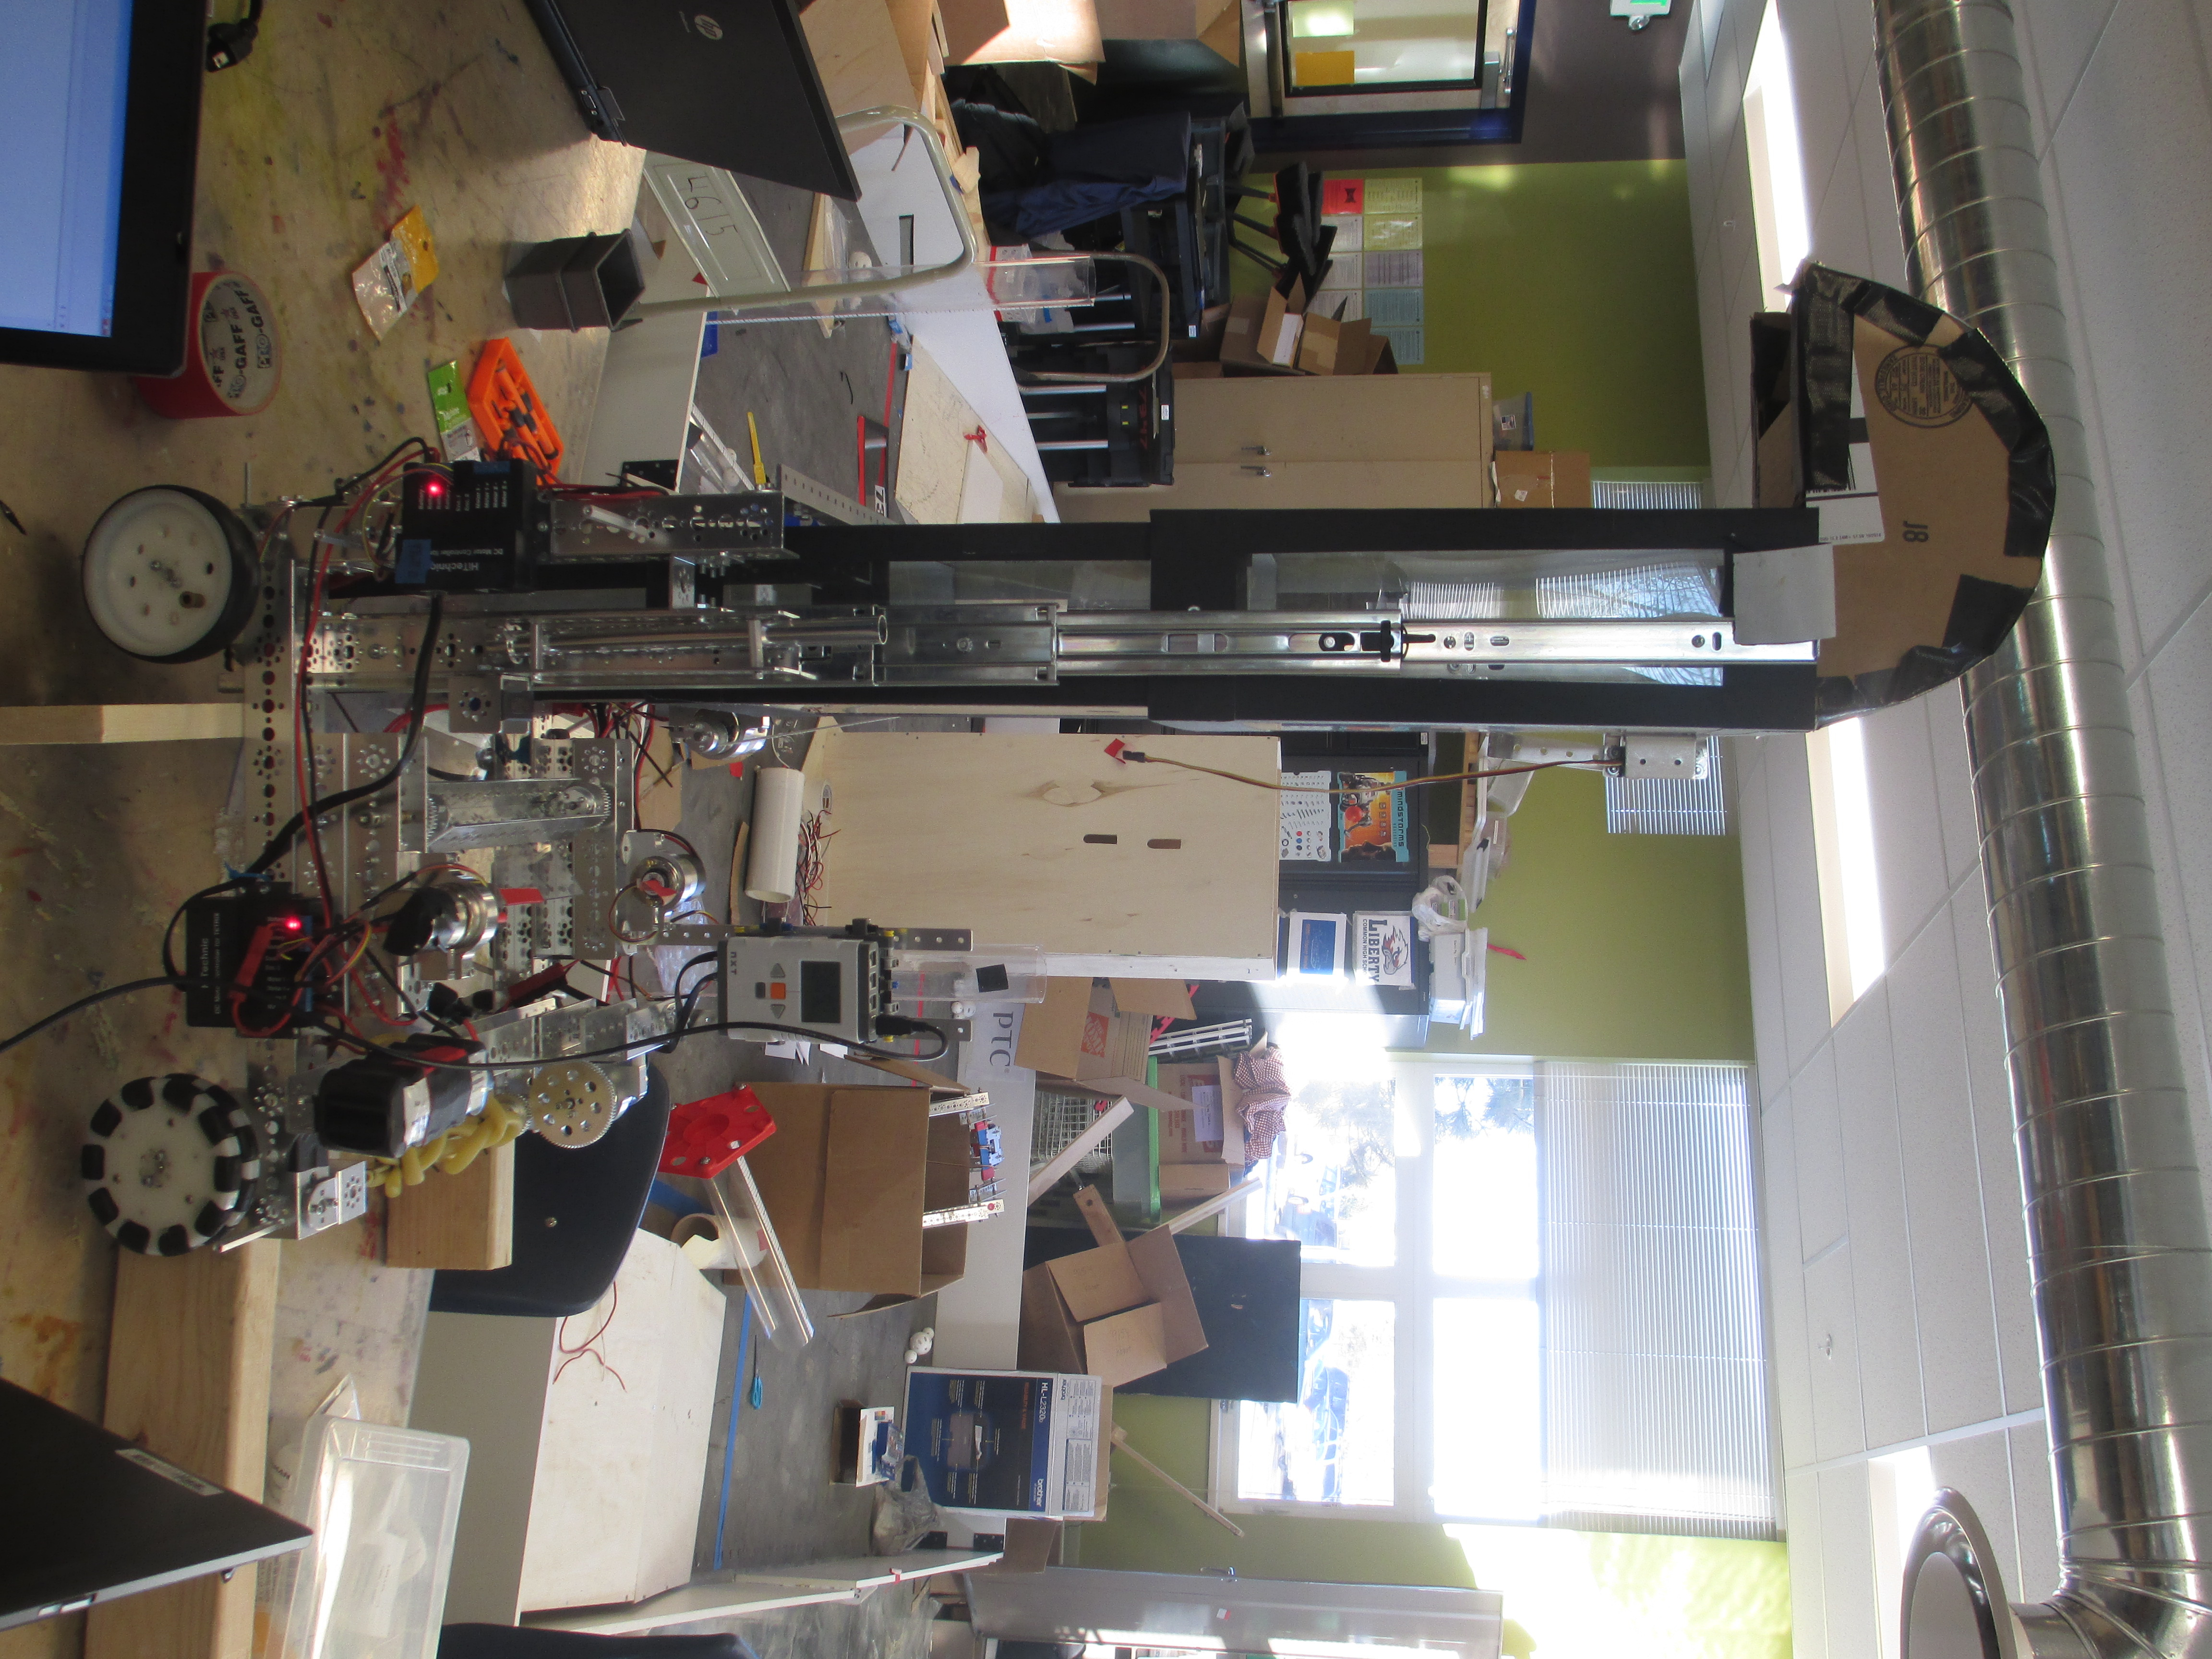
\includegraphics[height=7cm,angle=90]{./Entries/Images/robotFeb24.JPG}
\end{center}

Here is a close-up of the new deflector:

\begin{center}
 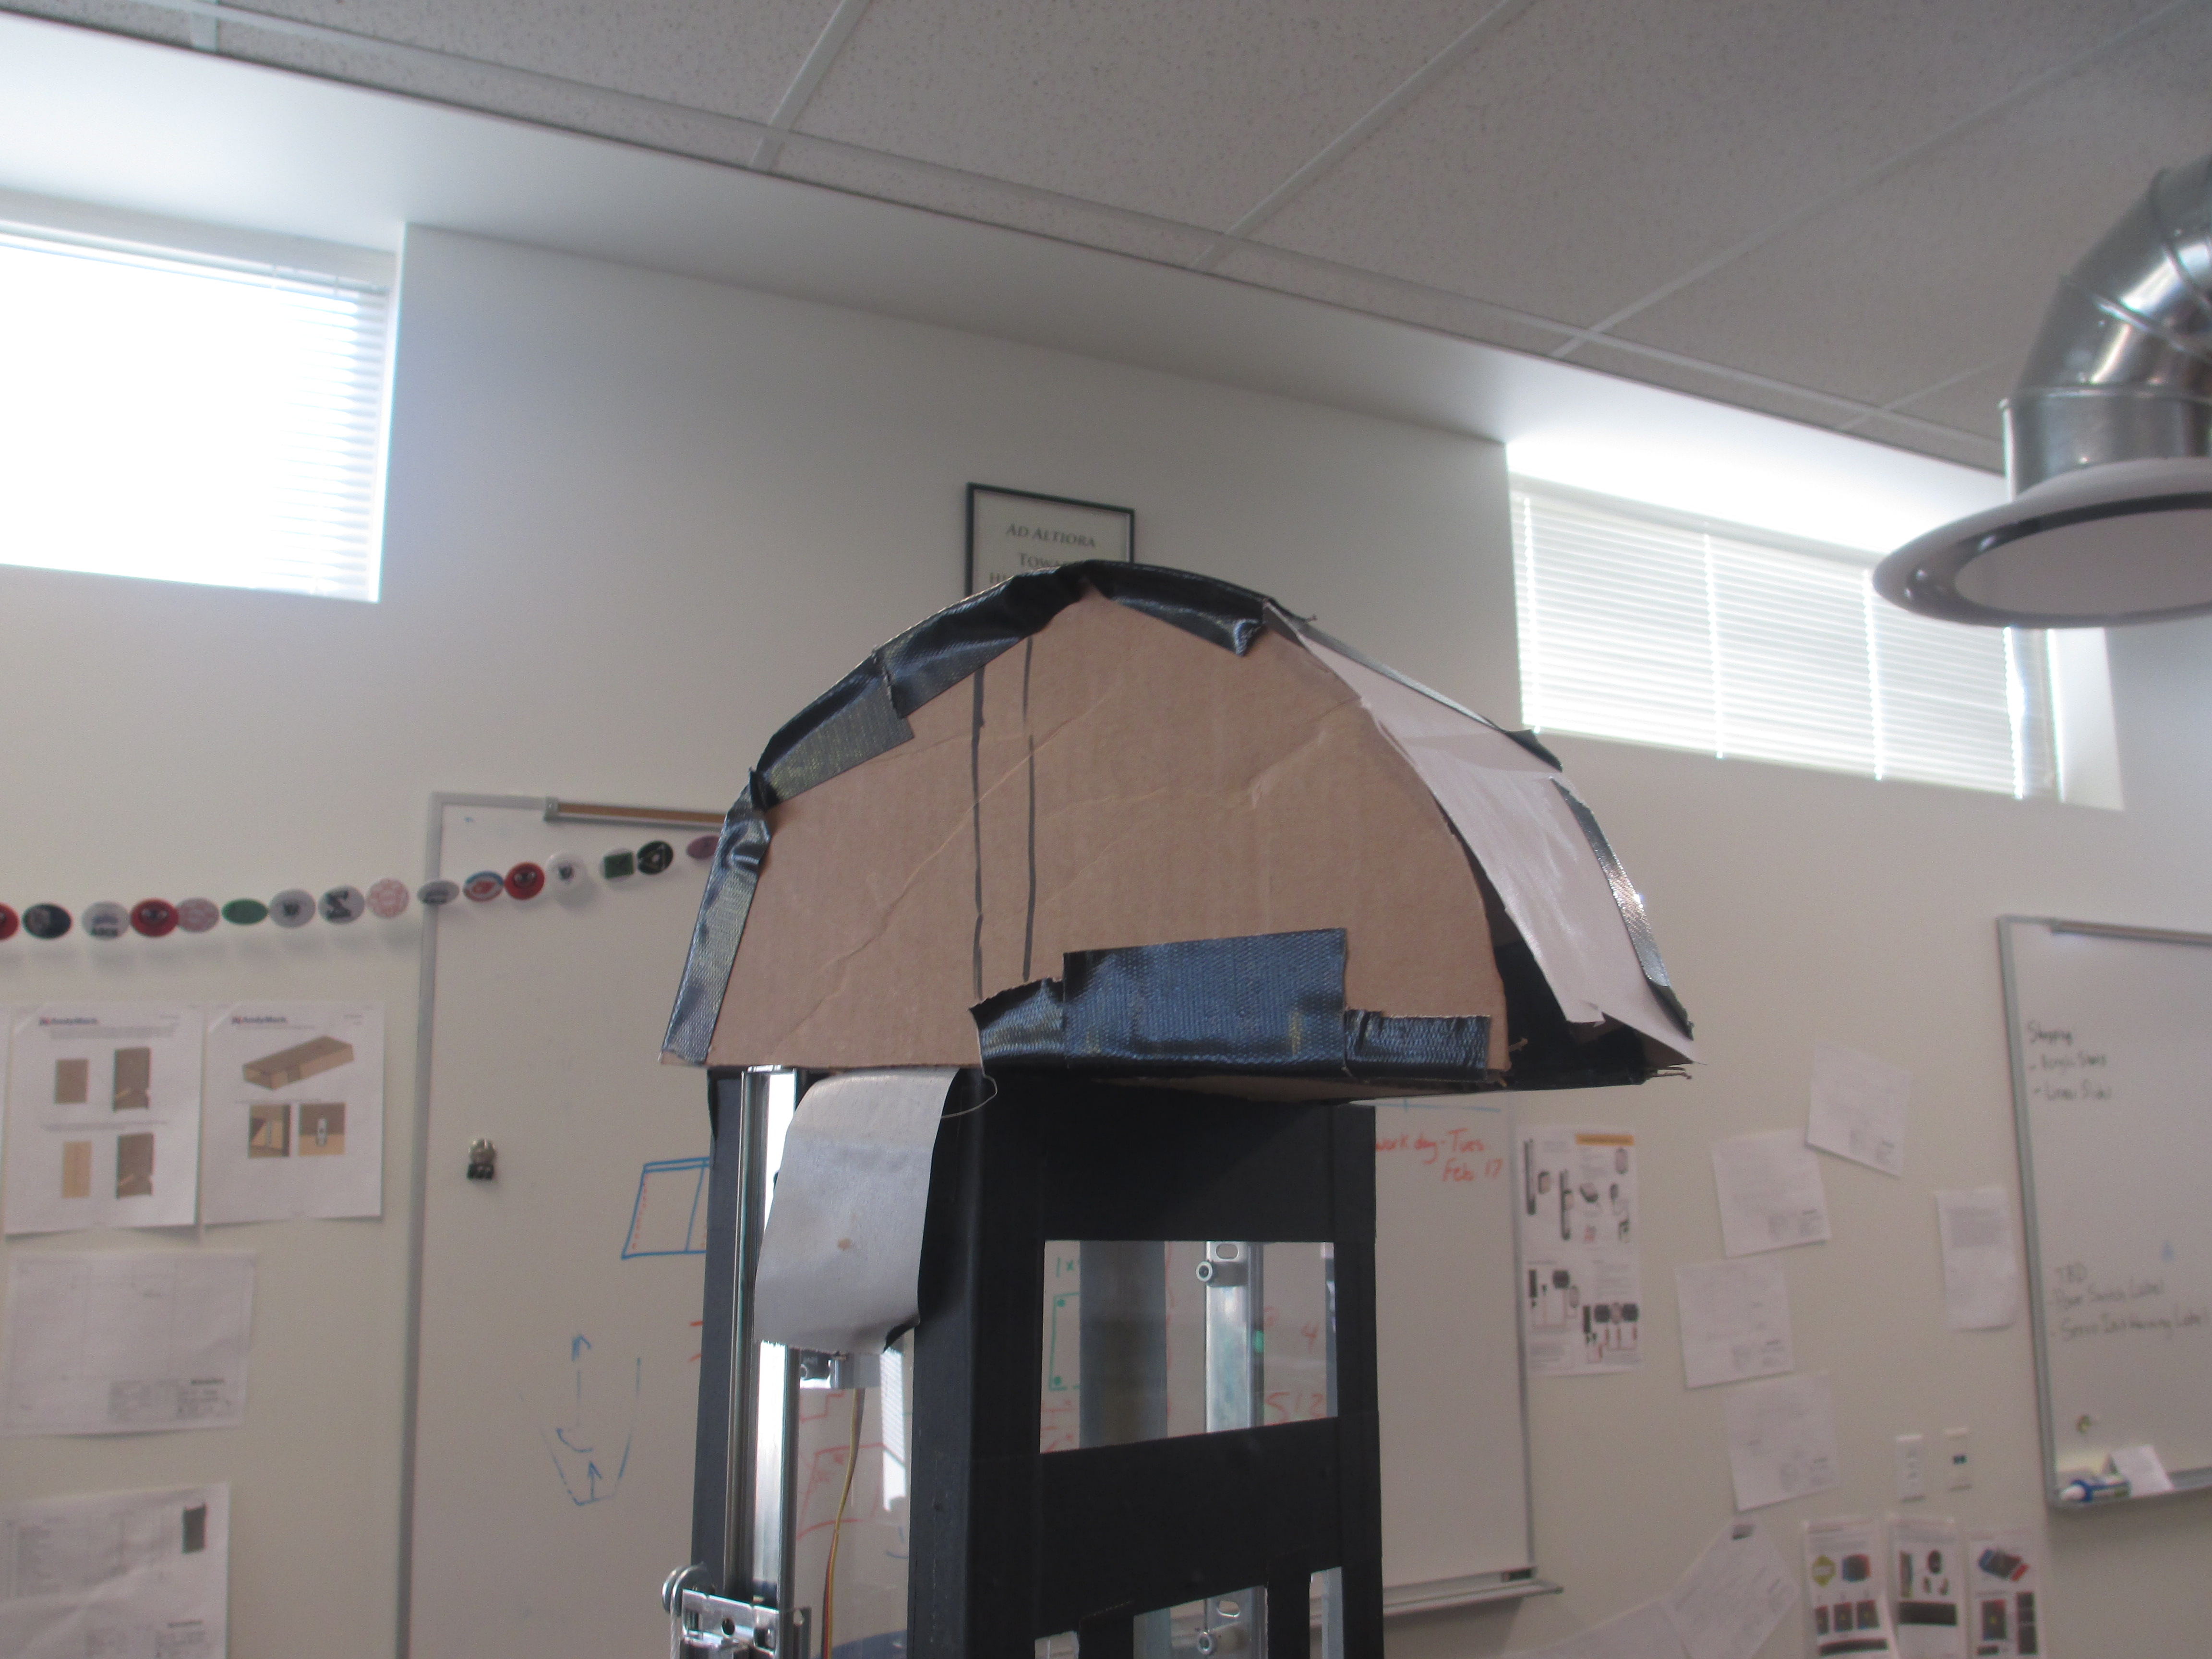
\includegraphics[height=6cm]{./Entries/Images/newDeflectorPrototype.JPG}
\end{center}

It is still in a prototype stage, but Filip and Matt are working on a polycarb version.

\pagebreak

Update 2015-02-26: Here is a picture of Filip and Matt's new deflector:

\begin{center}
 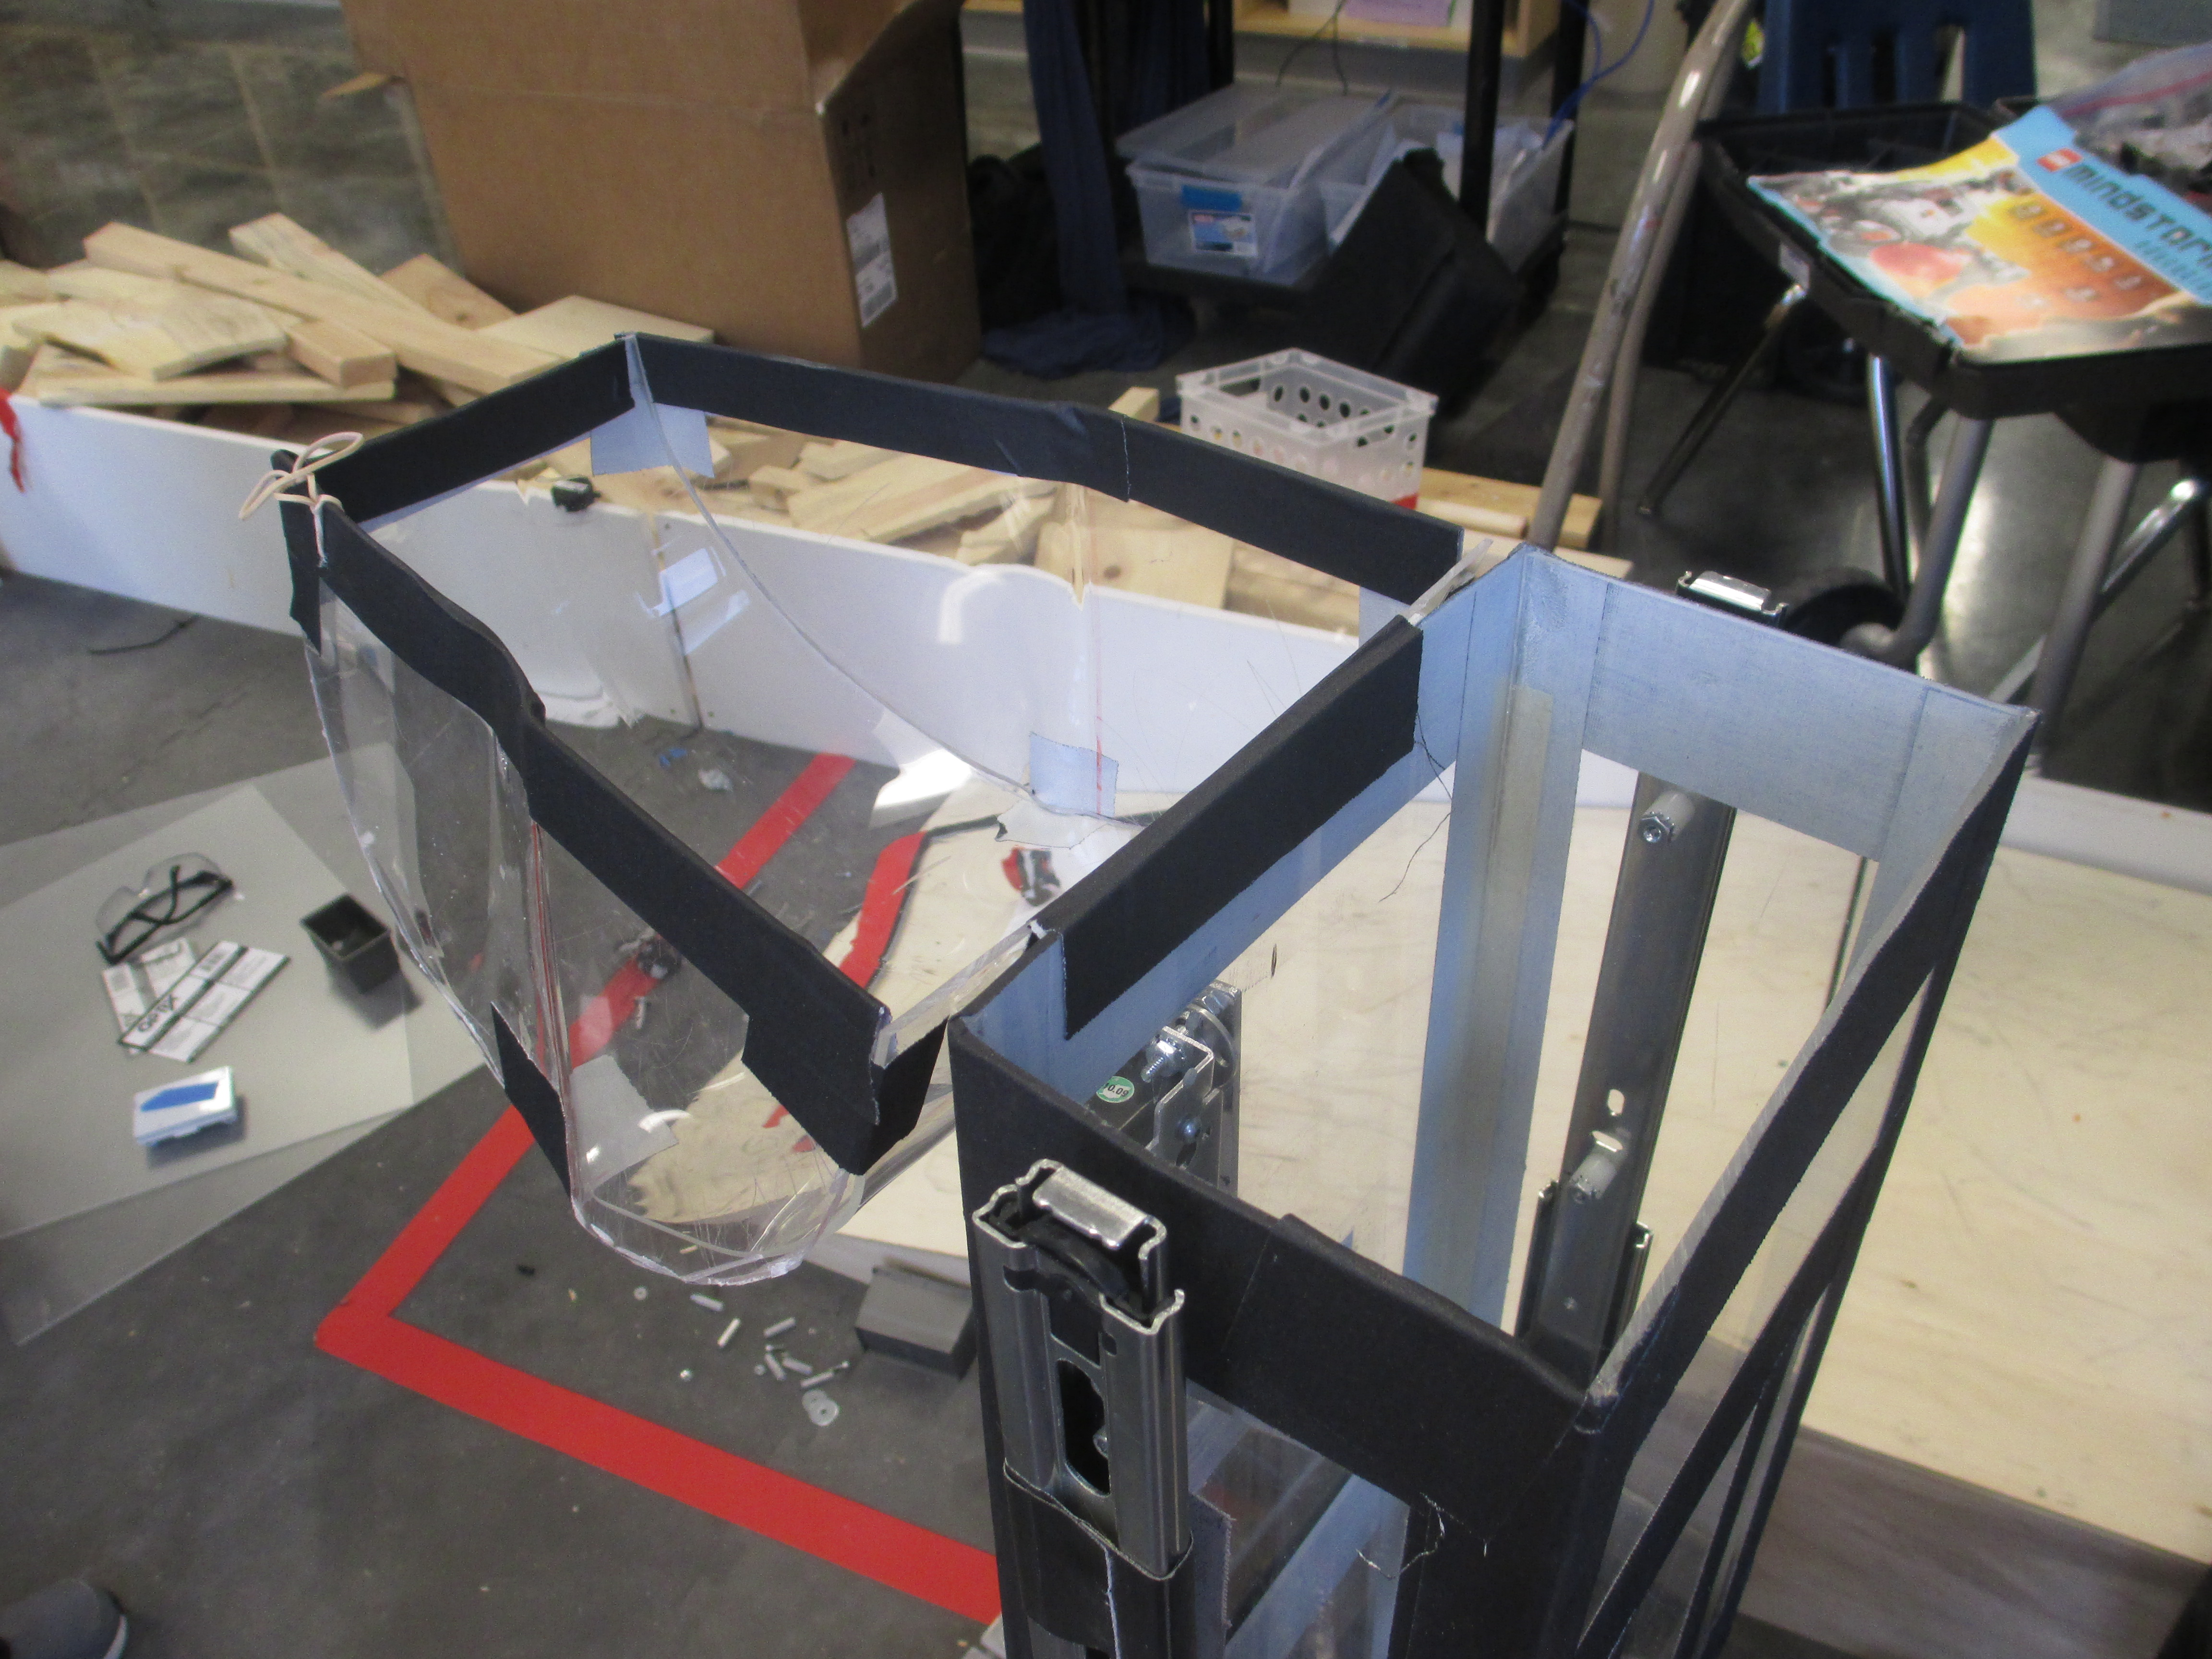
\includegraphics[width=\textwidth]{./Entries/Images/FinalDeflectorFeb26.JPG}
\end{center}
